%-----------------------------------------------------------------------
%  manuscript_aa.tex
%  Skeleton in Astronomy & Astrophysics format (aa.cls v9.4).
%
%  Contains ONLY: introduction, section/subsection titles, the numbered
%  equations, and Figs. 3 and 4 of manuscript_13page with their captions.
%
%  Compile with:  pdflatex manuscript_aa
%                 bibtex   manuscript_aa
%                 pdflatex manuscript_aa   (x2)
%-----------------------------------------------------------------------

\documentclass{aa}

\usepackage{graphicx}
\usepackage{txfonts}
\usepackage{amsmath}
\usepackage[colorlinks=true,citecolor=blue,linkcolor=blue,urlcolor=blue]{hyperref}

% --- shorthands carried over from manuscript_13page -------------------
\newcommand{\Ke}{K_{\mathrm{e}}}
\newcommand{\Ki}{K_{\mathrm{ini}}}
\newcommand{\zi}{z_{\mathrm{i}}}
\newcommand{\xHI}{x_{\mathrm{HI}}}

\begin{document}

   \title{Cosmic-ray electrons as ionizing agents of the intergalactic
          medium during the epoch of reionization}

   \subtitle{}

   \author{L. Carvalho \inst{1}\corrauth{lautarocarvalho@gmail.com}
        \and L. J. Pellizza \inst{1}
        \and G. J. Escobar \inst{1}
        }

   \institute{Instituto de Astronom\'{\i}a y F\'{\i}sica del Espacio
              (IAFE), CONICET--UBA, Buenos Aires, Argentina}

   \date{Received ; accepted }

  \abstract
  % context
   {}
  % aims
   {}
  % methods
   {}
  % results
   {}
  % conclusions
   {}

   \keywords{intergalactic medium --
             dark ages, reionization, first stars --
             cosmic rays --
             radiation mechanisms: non-thermal
            }

   \maketitle

%%%%%%%%%%%%%%%%%%%%%%%%%%%%%%%%%%%%%%%%%%%%%%%%%%%%%%%%%%%%%%
\section{Introduction}
\label{sec:intro}

The epoch of reionization (EoR) was the global phase transition of the
primordial neutral hydrogen into an ionized state. This process started with
the cosmic dawn (CD), when the first sources of stellar light were formed the radiation emitted by them began to heat and ionize the surrounding medium, since redshift $z \sim 30$ \citep{Bromm2013,Klessen2023}. At the other end, observations of the Ly$\alpha$ forest indicate that reionization-related fluctuations were still present at $z \simeq 5.3$, and the Thomson scattering optical depth of the CMB, $\tau = 0.054 \pm 0.007$, constrains the midpoint of this process aroud $z \simeq 7.7$ \citep{Bosman2022,Planck2020}. Therefore, the range $5.5 \le z \le 30$ contains
the interval of cosmic time in which the reionization of the intergalactic medium (IGM) takes process
\citep{Robertson2022,Klessen2023}.


Star-forming galaxies are widely considered to be the main sources of ionizing radiation \citep{Robertson2022}, but the
abundances and ionizing efficiencies inferred from \emph{JWST} are high enough that the, with the estimated values for escape fraction, they would complete reionization too early \citep{Munoz2024}. A budget that is over-supplied in photons is precisely the situation in which the secondary, non-stellar channels of energy injection deserve to be quantified rather than assumed negligible.

The presence of cosmic rays (CR) has been  tightly linked to the life-cycle of stellar populations. Stellar winds, accretion events, supernova explosions, neutron stars and high-mass X-ray binaries are well-established accelerators of both hadronic and leptonic CRs via collisionless shocks, with
kinetic particle-in-cell simulations showing that electrons and protons are injected together at quasi-parallel shocks
\citep{Aharonian2019,Park2015} \citep{Bykov2017}
\citep{Mirabel2011,Kaur2022}. Because these engines all appear within a few million years of the first star formation, CRs have been present throughout the entirety of the EoR, interacting with the primordial IGM and injecting energy into it \citep{Sazonov2015,Leite2017,Ruszkowski2023}.

For that injected energy to affect the IGM the particles must first leave the object that accelerated them. \textcolor{red}{The early Universe may favours this: minihaloes have shallow potential wells, short magnetic confinement times and low column densities, and the photoevaporation that accompanies the first ionizing sources removes much of the confining gas, so
that CRs produced by the first supernova remnants are released essentially directly into the surrounding neutral medium
\citep{Sazonov2015,Leite2017,Jana2018}.} 

The relevant configuration is therefore a relativistic particle propagating in a diffuse, cold and almost fully neutral IGM, and the question becomes how it deposits its kinetic energy there.

That deposition occurs as a cascade: high-energy CR electrons and photons trigger extensive electromagnetic showers, in which each generation of secondary particles are capable of ionize, excite and produce further generations of particles \citep{Valdes2010,Slatyer2016}. 

For high-energy electrons ($K_{\mathrm{e}} \gtrsim 1 \text{MeV}$), the dominant energy loss mechanism is inverse Compton (IC) scattering off the dense CMB \citep{Blumenthal1970,Gould1972}, whose energy density grows as $(1+z)^{4}$, surpassing every other channel at equal redshifts.  However, the up-scattered photons are only useful for reionization within a certain energy window: the parent electron must be energetic enough for the scattered photon to exceed the $13.6\ \mathrm{eV}$ threshold, but not so much that the resulting photon has a mean free path against photoionization longer than the Hubble radius, in which case it free-streams
away \citep{Zdziarski1989,Slatyer2016}. \textcolor{red}{Locating these boundaries quantitatively is one of the aims of this work.}

For low-energy electrons ($K_{\mathrm{e}} \lesssim 100 \text{keV}$) the main cooling mechanism is instead the collisional ionization of the cold neutral hydrogen. This converts the electron energy directly into free electrons \citep{KimRudd1994,Kim2000}, which eventually
thermalize when their energy falls below $10.2\ \mathrm{eV}$ and can no longer ionize nor excite more atoms; it then injects its remaining energy into the IGM via atomic Coulomb collisions with the residual free electrons \citep{Shull1985,Furlanetto2010}.

Heating and ionization are thus not independent processes but two branches of the same energy budget, reinged over by the same cross-sections. 

The HERA Phase~I 21-cm power-spectrum limits require the IGM to have been warmed above the adiabatic cooling floor no later than $z = 10.4$ \citep{HERA2023,Mertens2025}. What remains to be established is how much of that energy comes from each different source.

\citet{Nath1993} asked directly whether CRs from young
galaxies could reionize or heat the IGM, and it has been revisited with progressively more complete microphysics ever since \citep{Samui2005,Sazonov2015,Leite2017,Jana2018,Bera2023,GesseyJones2023}. The literature point mainly towards the heating effect of CR and found it to be substantial, reaching $\Delta T \simeq 10$--$200\ \mathrm{K}$ by $z = 10$ \citep{Sazonov2015,Leite2017}, whereas the ionization is concluded to be negligible \citep{Leite2017}. However, most works exclusively aboard the hadronic component, which carries the bulk of the CR energy budget. The electronic component interacts via completely different channels, IC scattering on the CMB above all, which is suppressed for protons by $(m_e/m_p)^{4} \simeq 10^{-13}$ and is therefore irrelevant for hadrons, but dominate for electrons above $\sim\!100\ \mathrm{keV}$.


In this work, we extensively analyze and discuss the most relevant phenomena that affect the CR electron propagation and energy deposition through the EoR. We focus mainly on the cooling mechanisms by which CR electrons can heat and ionize the early IGM, evaluate their efficiency, and determine the optimal parameters for which those electrons could have contributed to the global reionization of the Universe. Finally, we discuss
which astrophysical scenarios could feasibly produce CR electrons within the found optimal parameter space to change the thermodynamic state of the IGM.


%%%%%%%%%%%%%%%%%%%%%%%%%%%%%%%%%%%%%%%%%%%%%%%%%%%%%%%%%%%%%%
\section{Physical model}
\label{sec:model}

\subsection{Fiducial IGM}
\label{sec:igm}

\begin{equation}
   n_{\mathrm{HI}}(z) = 1.8\times10^{3}
   \left(\frac{1+z}{21}\right)^{3}\ \mathrm{m^{-3}},
   \qquad
   x_e \equiv \frac{n_e}{n_{\mathrm{HI}}} = 10^{-4} ,
   \label{eq:igm}
\end{equation}

\begin{equation}
   \frac{U_B}{U_{\mathrm{CMB}}}
   = \frac{B_0^{2}}{2\mu_0 U_{\mathrm{CMB},0}}
   = 9.5\times10^{-8} .
   \label{eq:ubucmb}
\end{equation}

\subsection{Seven simultaneous electron losses}
\label{sec:losses}

\begin{equation}
   \frac{d\Ke}{dt} = -\sum_{j=1}^{7} L_j(z,\Ke) .
   \label{eq:loss}
\end{equation}

\begin{equation}
   L_{\mathrm{rad}} = \frac{4}{3}\,\sigma_T c\,U\,
   \frac{p^{2}c^{2}}{(m_ec^{2})^{2}} ,
   \qquad
   U = U_B \ \ \mathrm{or}\ \ U_{\mathrm{CMB}}F_{\mathrm{KN}}(b) .
   \label{eq:rad}
\end{equation}


%%%%%%%%%%%%%%%%%%%%%%%%%%%%%%%%%%%%%%%%%%%%%%%%%%%%%%%%%%%%%%
\section{Structure of the cooling problem}
\label{sec:structure}

\subsection{Regime boundaries}
\label{sec:bounds}

\subsection{Integrated energy budgets}
\label{sec:budgets}

%_____________________________________________________________
%   Fig. 3 of manuscript_13page
%-------------------------------------------------------------
   \begin{figure}[ht!]
   \centering
   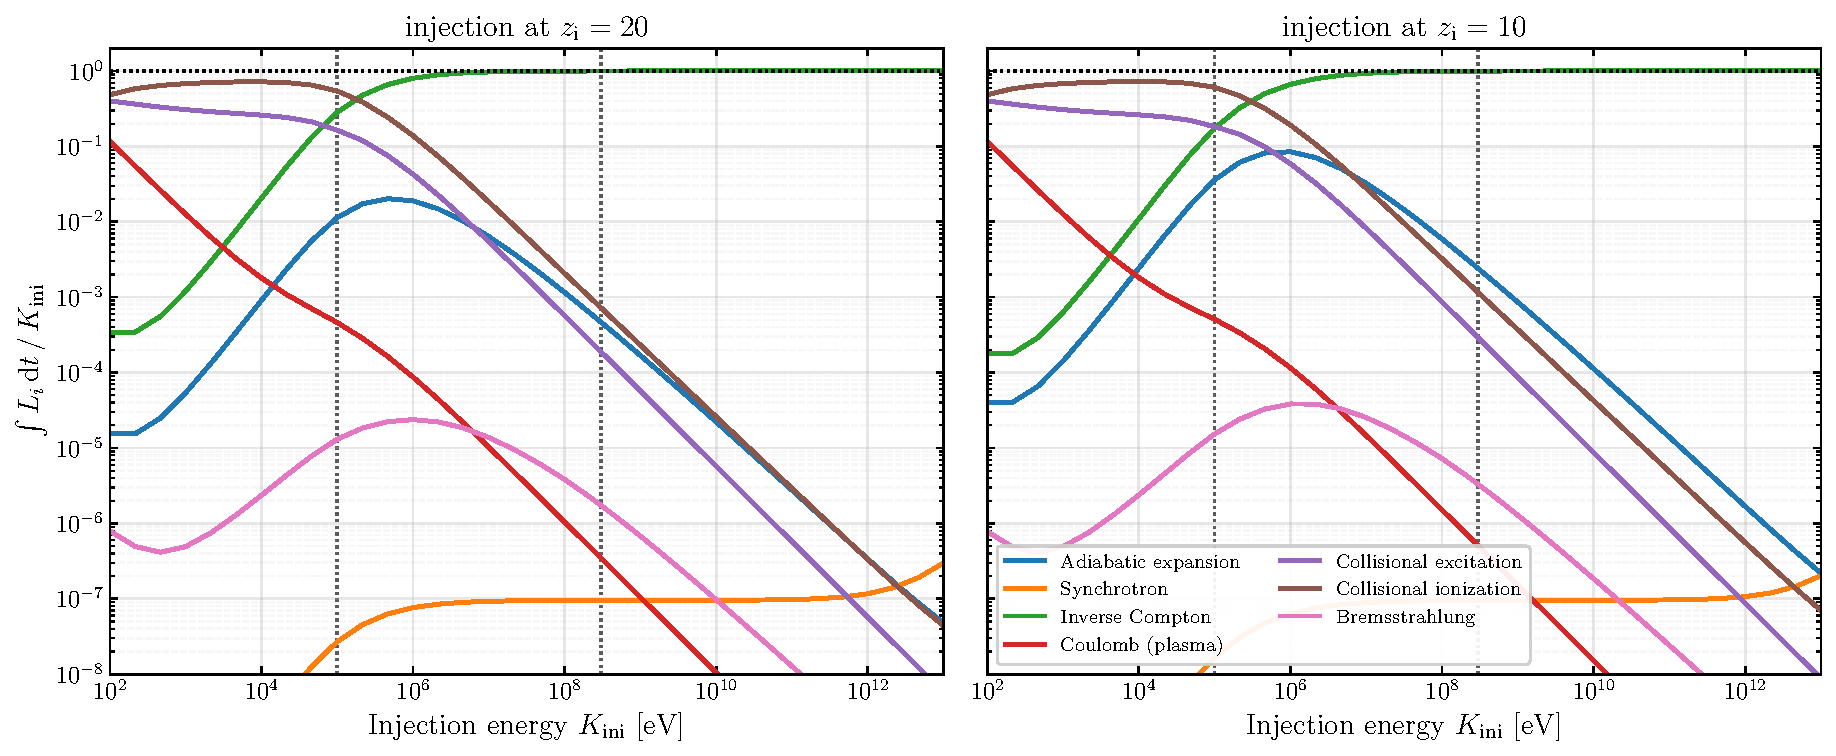
\includegraphics[width=\hsize]{fig04_energy_budget.pdf}
      \caption{Fraction of the injection energy carried by each electron-loss
      channel before thermalization, for $\zi=20$ and 10. IC energy in this
      figure is radiated energy; only the spectral fraction inside the adopted
      photon band is converted into ionizations in
      Sect.~\ref{sec:cascade}.}
         \label{fig:budget}
   \end{figure}


%%%%%%%%%%%%%%%%%%%%%%%%%%%%%%%%%%%%%%%%%%%%%%%%%%%%%%%%%%%%%%
\section{Ionization cascade}
\label{sec:cascade}

\subsection{Electron-impact branch}
\label{sec:ebranch}

\begin{equation}
   \dot Y_e = n_{\mathrm{HI}}\,v\,\sigma_{\mathrm{ion}}(\Ke)
   + ... .
   \label{eq:electron}
\end{equation}

\subsection{Productive inverse-Compton photons}
\label{sec:icbranch}

\begin{align}
   \frac{d\dot N_\gamma}{dE_\gamma}
   &= \frac{3\sigma_T c}{4\gamma^{2}}
      \int d\epsilon\,\frac{n(\epsilon)}{\epsilon}\,G(q,\Gamma) ,
      \label{eq:ic}\\
   q &= \frac{E_\gamma}{\Gamma(\gamma m_ec^{2}-E_\gamma)} ,
      \qquad
      \Gamma = \frac{4\gamma\epsilon}{m_ec^{2}} , \nonumber\\
   G &= 2q\ln q + (1+2q)(1-q)
      + \frac{(\Gamma q)^{2}(1-q)}{2(1+\Gamma q)} . \nonumber
\end{align} \cite{Blumenthal1970}

\begin{equation}
   \dot Y_\gamma = \int_{B_{\mathrm{H}}}^{E_{\max}} dE_\gamma\,
   \frac{d\dot N_\gamma}{dE_\gamma}
   \left[1 + Y_e(E_\gamma-B_{\mathrm{H}},z)\right] .
   \label{eq:photon}
\end{equation}
\textcolor{red}{
\begin{equation}
   \lambda_\gamma^{-1} = n_{\mathrm{HI}}\sigma_{\mathrm{pi}}(E_\gamma)
   + (n_{\mathrm{HI}}+n_e)\sigma_{\mathrm{KN}}(E_\gamma)
   = \frac{H(z)}{c} .
   \label{eq:mfp}
\end{equation}
}

%%%%%%%%%%%%%%%%%%%%%%%%%%%%%%%%%%%%%%%%%%%%%%%%%%%%%%%%%%%%%%
\section{Ionization results}
\label{sec:results}

%_____________________________________________________________
%   Fig. 4 of manuscript_13page
%-------------------------------------------------------------
   \begin{figure}[ht!]
   \centering
   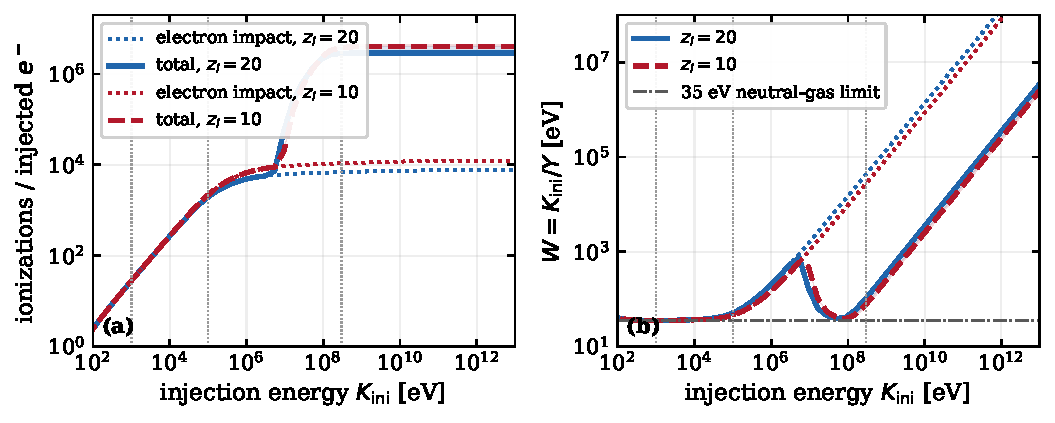
\includegraphics[width=\hsize]{fig_photon_yield.pdf}
      \caption{\textbf{(a)} Ionizations per injected electron. Dotted curves
      show the electron direct ionization events; thick curves add IC photons in the
      13.6 eV--1 keV band and their photoionization events.
      \textbf{(b)} Effective energy per ionization. The first minimum is the
      low-energy collisional cascade and the second is the IC-photon window.}
         \label{fig:yield}
   \end{figure}

\subsection{The direct collisional window}
\label{sec:window1}

\subsection{The IC-photon window}
\label{sec:window2}


%%%%%%%%%%%%%%%%%%%%%%%%%%%%%%%%%%%%%%%%%%%%%%%%%%%%%%%%%%%%%%
\section{Cooling histories and spatial interpretation}
\label{sec:histories}


%%%%%%%%%%%%%%%%%%%%%%%%%%%%%%%%%%%%%%%%%%%%%%%%%%%%%%%%%%%%%%
\section{Injection spectra and global scaling}
\label{sec:global}



%%%%%%%%%%%%%%%%%%%%%%%%%%%%%%%%%%%%%%%%%%%%%%%%%%%%%%%%%%%%%%
\section{Discussion and limitations}
\label{sec:discussion}


%%%%%%%%%%%%%%%%%%%%%%%%%%%%%%%%%%%%%%%%%%%%%%%%%%%%%%%%%%%%%%
\section{Conclusions}
\label{sec:conclusions}


%%%%%%%%%%%%%%%%%%%%%%%%%%%%%%%%%%%%%%%%%%%%%%%%%%%%%%%%%%%%%%
% Sources of the equations above, kept in the reference list so that
% Sects. 2-7 can be written without re-hunting them.
\nocite{Astropy2022,Stone2002,Karzas1961,Slatyer2009}

\bibliographystyle{aa}
\bibliography{references}

\end{document}
